\documentclass[12pt,a4paper,UTF8]{article}
\usepackage{ctex} % Chinese support
\usepackage{graphicx} % Insert images
\usepackage{listings} % Print source code
\usepackage{color} % Color support
\usepackage{booktabs} % Professional table support
\usepackage{pdflscape} % Landscape pages support in PDF
\usepackage{hyperref} % Hypertext links support for cross-referencing

% Customize hyperref format (it's set to no special format here)
\hypersetup{hidelinks}

% Declare directories to search for graphics files for graphicx
\graphicspath{{figures/}{logo/}}

% Define source code style for listings
\lstdefinestyle{python}{
  language=Python,
  basicstyle=\ttfamily\footnotesize,
  keywordstyle=\bfseries\color[rgb]{0, 0, 1},
  identifierstyle=\color[rgb]{0.5, 0.3, 0.1},
  stringstyle=\color[rgb]{0.6, 0.1, 0.1},
  commentstyle=\itshape\color[rgb]{0.05, 0.5, 0.05},
  backgroundcolor=\color[gray]{0.95},
  numbers=left,
  numbersep=5pt,
  numberstyle=\color[gray]{0.6},
  breaklines=true
}

% Define new command for title page
\newcommand{\reporttitle}[2]{
  \LARGE\textsf{#1}\quad\underline{\makebox[12em]{#2}}
}
\newcommand{\reportinfo}[2]{
  \large\makebox[4em]{\textsf{#1}}\quad\underline{\makebox[18em]{#2}}
}

% The document begins here
\begin{document}
\begin{titlepage}
  \centering
  \vspace*{\fill}
  
\includegraphics[height=144pt]{nju-logo}\\[48pt]
  {\huge\textsf{课\ 程\ 实\ 验\ 报\ 告}}\\[48pt]
  \reporttitle{实验名称}{Switchyard \& Mininet}\\[72pt]

  \reportinfo{课程名称}{计算机网络}\\[8pt]
  \reportinfo{院\hspace{\fill}系}{计算机科学与技术系}\\[8pt]
  \reportinfo{学\hspace{\fill}号}{191220129}\\[8pt]
  \reportinfo{姓\hspace{\fill}名}{邢尚禹}\\[8pt]
  \reportinfo{邮\hspace{\fill}箱}{191220129@smail.nju.edu.cn}\\[8pt]
  \reportinfo{实验日期}{2021年3月}\\
  \vspace*{\fill}
\end{titlepage}

\tableofcontents
\newpage

\section{实验目的}
\begin{itemize}
	\item 学习linux, python, git, vscode等工具的基本使用;
	\item 学习使用mininet搭建模拟网络;
	\item 学习使用wireshark抓包;
	\item 学习使用switchyard实现硬件逻辑。
\end{itemize}

\section{实验内容}
\begin{enumerate}
	\item 安装并配置linux, python, git, vscode等工具;
	\item 了解mininet,wireshark和switchyard的使用方法;
	\item 对指定的代码进行修改,以完成特定的功能。
\end{enumerate}

\section{实验过程及结果}
task 1,2,3此处略过,本节仅简述task 4的实验过程和结果。

\subsection{Modify the Mininet topology}
选择第一个实现:删除server2,只需将start\_mininet.py的第30至33行的server2注释即可。
\lstinputlisting[style=python]{1.py}
修改后的结构为:server1 --- hub --- client

\subsection{Modify the logic of a device}
要实现接受和发送的包的数量统计,只需要添加全局变量in\_count和out\_count,接受和发送时分别+1即可。
在循环的最后,通过log\_info函数格式化字符串输出。
\lstinputlisting[style=python]{2.py}
在mininet CLI中执行server1 ping 192.168.100.3 -c 1命令,在switchyard中得到如下log:
\begin{figure}[htbp]
	\centering
	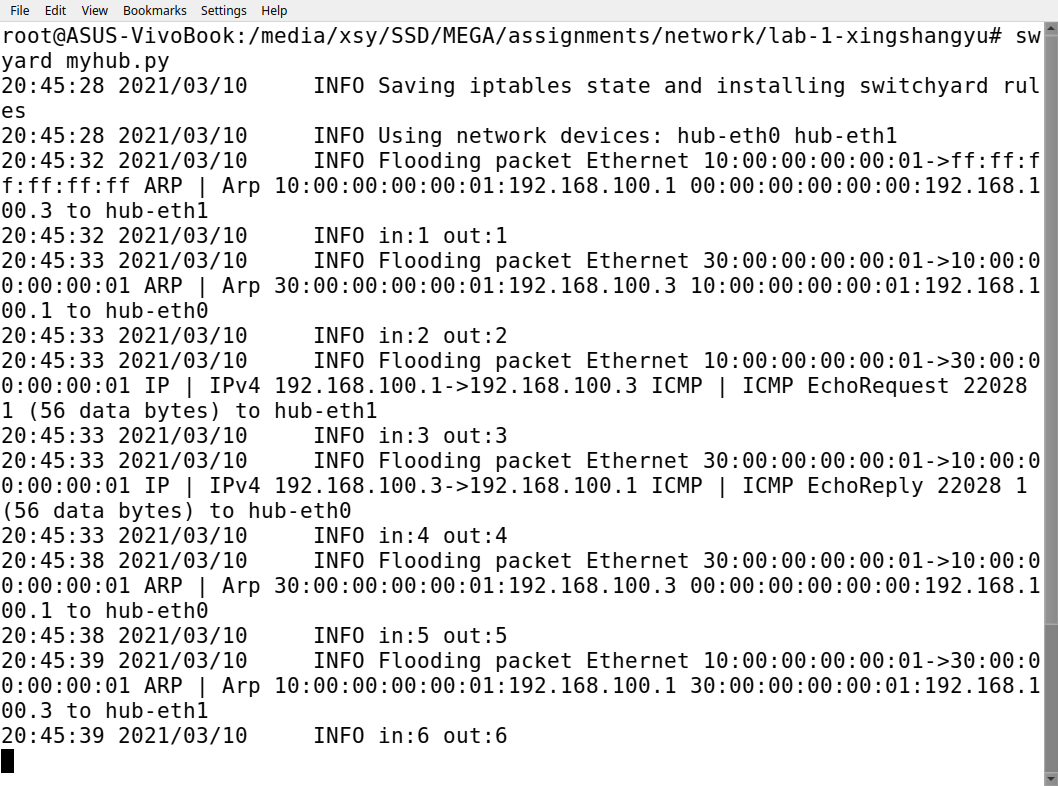
\includegraphics[width=\textwidth]{hublog}
	\caption{hublog}
\end{figure}

\newpage
\subsection{Modify the test scenario of a device}
通过调用new\_packet函数,添加一个测试:client向hub发送一个frame。根据hub的逻辑,
不会出现任何包的转发。在最后一个expect语句前添加如下代码:
\lstinputlisting[style=python]{3.py}
测试结果:
\begin{figure}[htbp]
	\centering
	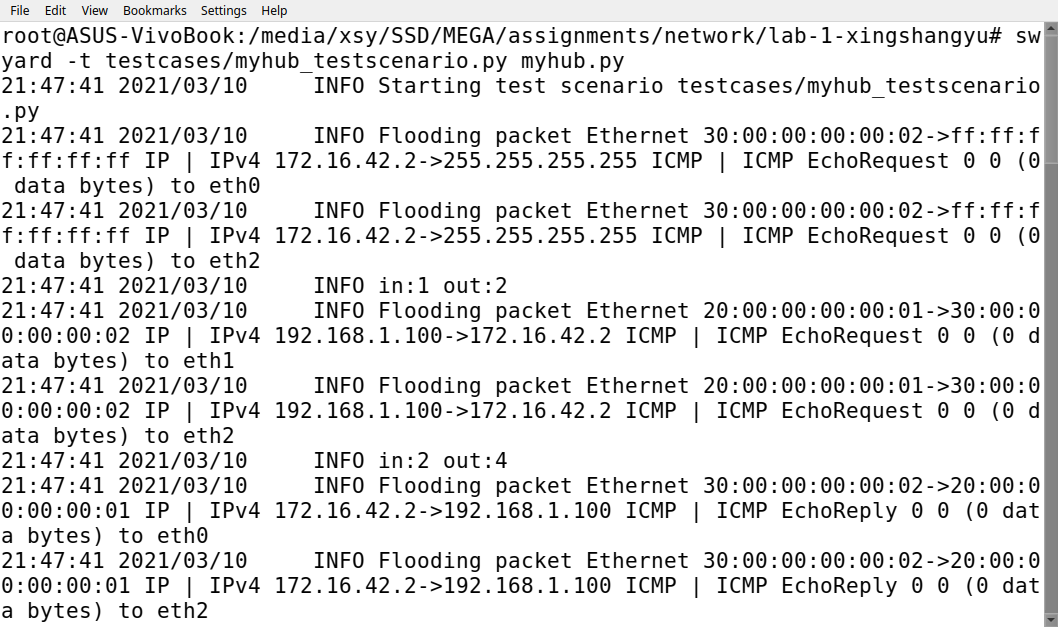
\includegraphics[width=\textwidth]{hub_test_1}
	\caption{hubtest\_1}
\end{figure}
\begin{figure}[htbp]
	\centering
	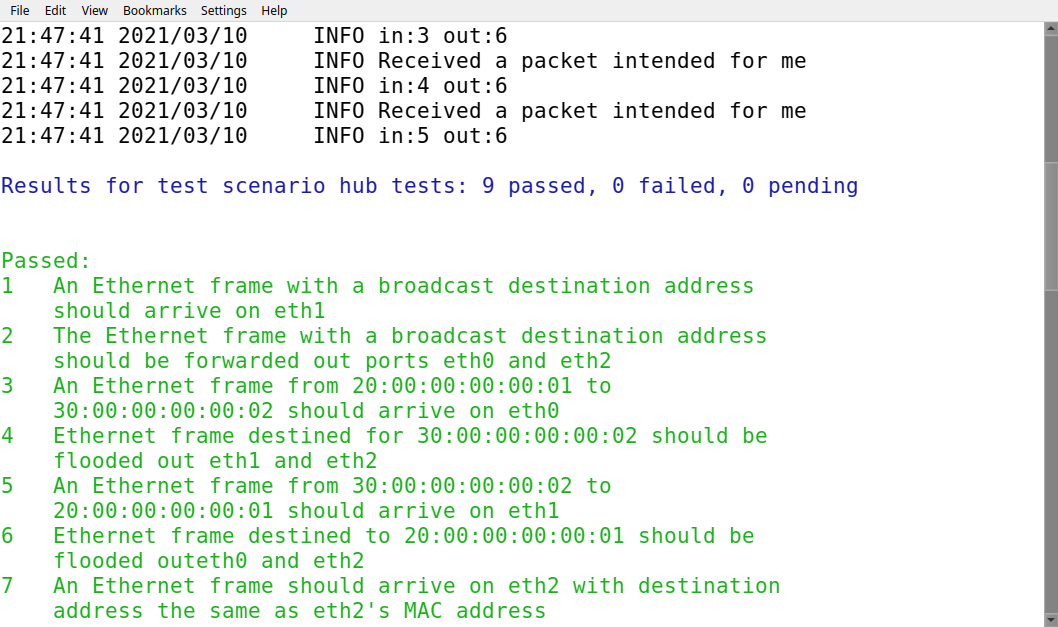
\includegraphics[width=\textwidth]{hub_test_2}
	\caption{hubtest\_2}
\end{figure}
\begin{figure}[htbp]
	\centering
	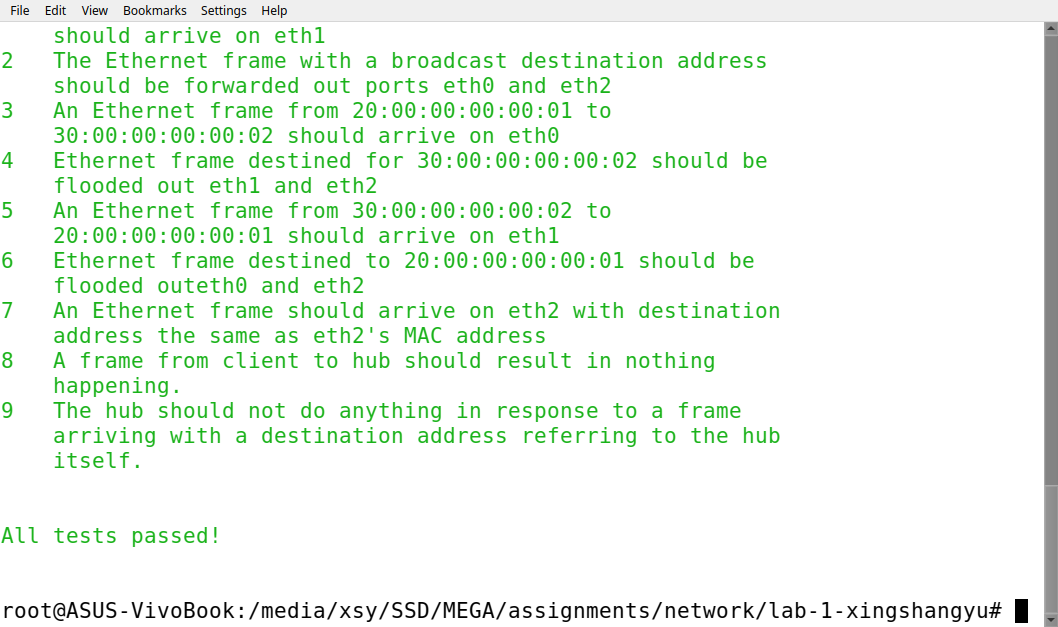
\includegraphics[width=\textwidth]{hub_test_3}
	\caption{hubtest\_3}
\end{figure}

\newpage
\subsection{Run your device in Mininet}
运行步骤:
\begin{enumerate}
	\item 运行mininet:sudo python3 start\_mininet.py
	\item 运行hub switchyard:hub xterm \&,在xterm中运行switchyard:swyard myhub.py
	\item 在mininet中生成一些traffic,这里让server1 ping client:server1 ping 192.168.100.3 -c 1
\end{enumerate}

\subsection{Capture using Wireshark}
运行上述前2步后,运行wireshark:client wireshark。然后让client ping server得到6个包,记录见文件capture.pcnpng。
捕获得的包为:
\begin{enumerate}
	\item client询问server的mac address;
	\item 回应server的mac address;
	\item client向server发送ping request;
	\item server询问client的mac address;
	\item 回应server的mac address;
	\item server向client发送ping reply。
\end{enumerate}

\section{总结与感想}
\begin{itemize}
	\item 做实验前要先了解相关工具的使用,可以事半功倍;
	\item 英文阅读能力很重要。
\end{itemize}

\end{document}